% !TEX root = ../thesis-example.tex
%
\chapter{Natural Language Processing}
\label{sec:nlp}
In diesem Kapitel werden der theoretische Hintergrund und die Methoden des Natural-Language-Processings eingeführt. Nach den Grundlagen werden zwei verschiedene Methoden zum Parsen vorgestellt. Sofern nicht anders gekennzeichnet wurden die folgenden Abschnitte entnommen aus \cite{nlpGrundlagen}.

\section{Grundlagen}
\label{sec:nlp:grundlagen}

Betrachtet wird ein Satz einer natürlichen Sprache, die im Rahmen dieser Arbeit auf Englisch festgelegt ist. Als Satz wird hier eine Folge von mindestens einem Wort einer Sprache gesehen. Dieser wird durch ein Satzzeichen abgeschlossen.
Ein Algorithmus kann einen natürlich-sprachlichen Satz nicht ohne Weiteres interpretieren. Hierfür bedarf es verschiedener Hilfsstrukturen und zusätzlicher Informationen.\\
Als ersten Schritt bietet es sich an, den einzelnen Wörtern eines Satzes ihre Wortart zuzuordnen. Mit Wortart, alternativ auch Wortklasse oder im Englischen \textit{part-of-speech} (POS), ist gemeint, wie ein Wort im Satz auftritt. Beispiele für Wortarten sind Nomen, Verb und Adjektiv. \\
Für die verschiedenen Wortklassen gibt es Abkürzungen, genannt \textit{Tags}. Jedem Wort der Sprache kann mindestens ein \textit{Tag} zugewiesen werden. In dieser Arbeit wird das \textit{Tagset}, die Menge an Wortarten aus der \textit{Penn-Treebank}, verwendet. Aufgelistet sind diese in Tabelle \ref{tab:pos-tags}. 

\begin{table}
\begin{tabular}{ | l l l |}
	\hline
	\multicolumn{3}{|c|}{Penn-Treebank Part-of-Speech Tags} \\
	\hline
	\hline
	Tag & Beschreibung & Beispiel \\
	\hline
	CC & Koordinierende Konjunktion & \textit{and} \\
	CD & Kardinalzahl & \textit{third}\\
	DT & Artikel & \textit{the}\\
	EX & Existentielles \textit{there} & \textit{there} is\\
	FW & Fremdword & \textit{les}\\
	IN & Präposition, unterordnende Konjunktion & \textit{in}\\
	JJ & Adjektiv & \textit{green}\\
	JJR & Adjektiv, Komparativ & \textit{greener}\\
	JJS & Adjektiv, Superlativ & \textit{greenest}\\
	LS & Listenelement Markierung & \textit{1)}\\
	MD & Modal & \textit{could}\\
	NN & Nomen, singular oder Masse & \textit{table}\\
	NNS & Nomen, plural & \textit{tables}\\
	NNP & Eingenname, singular & \textit{Germany}\\
	NNPS & Eigenname, plural & \textit{Vikings}\\
	PDT & Predeterminer & \textit{both} his children \\
	POS & possesive Endung & \textit{'s} \\
	PRP & Personalpronomen & \textit{me} \\
	PRP\$ & Possesivpronomen & \textit{my} \\
	RB & Adverb & \textit{extremely} \\
	RBR & Adverb, Komparativ & \textit{better} \\
	RBS & Adverb, Superlativ & \textit{best} \\
	RP & Partikel & \textit{about} \\
	SYM & Symbol & \textit{\%} \\
	TO & to & what \textit{to} do \\
	UH & Ausruf & \textit{oops} \\
	VB & Verb, Grundform & \textit{be} \\
	VBD & Verb, Vergangenheitsform & \textit{was} \\
	VBG & Verb, Gerund \textbackslash Partizip Präsens & \textit{being} \\
	VBN & Verb, Partizip Perfekt & \textit{been} \\
	VBP & Verb, Präsens, nicht 3.Person Singular & \textit{am}  \\
	VBZ & Verb, Präsens, 3.Person Singular & \textit{is} \\
	WDT & \textit{wh}-Artikel & \textit{which} \\
	WP & \textit{wh}-Pronomen & \textit{who} \\
	WP\$ & \textit{wh}-Possesivpronomen & \textit{whose} \\
	WRB & \textit{wh}-Adverb & \textit{be} \\
	\hline
\end{tabular}
\caption{Penn-Treebank POS Tags \cite{ptbInformationen}} 
\label{tab:pos-tags}
\end{table}

Der Satz
\begin{quote}
My dog also likes eating sausage.
\end{quote}
würde mit diesem \textit{Tagset} folgendermaßen annotiert werden:
\begin{quote}
My/PRP\$ dog/NN also/RB likes/VBZ eating/VBG sausage/NN ./.
\end{quote}
Das maschinelle zuweisen von \textit{POS-Tags} geschieht über das sogenannte \textit{Tagging}. \\
Darüber hinaus zeigt sich, dass in der englischen Sprache mehrere Wörter eine \textit{Konstituente} bilden. Darunter versteht man eine Gruppe von Wörtern, die sich im Satz als Einheit verhalten. Ein Beispiel hierfür ist die Nominalphrase \textit{``My Dog''} oder die Verbalphrase \textit{``likes eating sausage''}. Für diese Einheiten gibt es wiederum eine Sammlung an \textit{Tags}, genannt \textit{syntaktische Tags}, wobei hier ebenfalls die der \textit{Penn-Treebank} verwendet werden. Eine Beschreibung dieser \textit{Tags} ist zu finden in Tabelle \ref{tab:phrase-tags}. Diese Einheiten bilden die syntaktischen Komponenten eines Satzes. Jede Konstituente hat ein \textit{Tag}, das beschreibt um welche Art es sich handelt, und eine Spanne, die angibt welche Wörter in der Konstituente enthalten sind. Die Konstituente, die den kompletten Satz enthält und selbst in keiner anderen Konstituente enthalten ist, wird in dieser Arbeit oberste Konstituente genannt. \\
Die Menge der Tags  kann durch eine Menge an relationalen Tags erweitert werden. Diese Tags liefern eine Zusatzinformation und werden an die eben vorgestellten angehängt. Zum Beispiel bekommt das Subjekt eines Satzes das Suffix \textit{-SBJ}. Das heißt aus einer Nominalphrase \textit{NP} wird, falls sie ein Subjekt ist, \textit{NP-SBJ} \cite{relationaltags}. Dieser Erweiterungssatz ist nicht Teil dieser Arbeit, wurde aber der Vollständigkeit halber erwähnt.
\begin{table}
\begin{tabular}{ | l p{7cm} p{4cm} |}
	\hline
	\multicolumn{3}{|c|}{Penn-Treebank Syntactic Tags} \\
	\hline
	\hline
	Tag & Beschreibung & Beispiel \\
	\hline
	S & einfacher deklarativer Satz & \textit{There we go.} \\
	SBAR & Satz beginnend mit unterordnender Konjunktion & feels \textit{like we have to move} \\
	SBARQ & Direkte Frage beginnend mit \textit{wh}-Wort oder \textit{wh}-Phrase & \textit{So what's that about?} \\
	SINV & Invertierter deklarativer Satz & neither \textit{am I a pessimist.} \\
	SQ & Invertierte Ja/Nein Frage oder Hauptsatz einer \textit{wh}-Frage & \textit{Will they move on?} \\
	
	ADJP & Adjektivphrase & \textit{relatively cheap} \\
	ADVP & Adverbphrase & \textit{down here} \\
	CONJP & Konjunktionalphrase &  \textit{but also for tissues}\\
	FRAG & Fragment & if \textit{not today}, ... \\
	INTJ & Zwischenruf &  \textit{Well} \\
	LST & Listenmarkierung & \textit{1} \\
	NAC & Keine Komponente & via the \textit{Freedom of Information} \\
	NP & Nominalphrase & \textit{the sun} \\
	NX & Markiert Kopf in komplexen NP & fresh \textit{apples and cinnamon} \\
	PP & Präpositionalphrase & \textit{in some way} \\
	PRN & Nebenläufige Phrase & \textit{..., bless his heart, ...} \\
	PRT & Partikel & \textit{up} \\
	QP & Quantifizierende Phrase & \textit{or two a day} \\
	RRC & Reduzierter Relativsatz & titles \textit{not presently in the collection} \\
	UCP & Ungleich Koordinierte Phrasen & She flew \textit{yesterday and on July 4th.} \\
	VP & Verbalphrase & this \textit{is my dog.} \\
	WHADJP	& \textit{Wh}-Adjektivphrase & \textit{how great you are} \\
	WHADVP & \textit{Wh}-Adverbphrase & \textit{When} I see it\\
	WHNP & \textit{Wh}-Nominalphrase & \textit{What} they've done \\
	WHPP & \textit{Wh}-Präpositional & \textit{At which} \\
	X & Unbekannt & \textit{The more} ..., \textit{the less} ... \\	
	
	\hline
\end{tabular}
\caption{Penn-Treebank syntaktische Tags \cite{penntagsetAusfuehrlich}} 
\label{tab:phrase-tags}
\end{table}
\\
In Abbildung \ref{fig:multiline-annotated-dog-eating} wird der Satz mit der syntaktischen Annotation dargestellt. Mit Annotation werden in dieser Arbeit die \textit{Tags} und Klammerungen bezeichnet. Ein Satz ist annotiert, wenn alle seine Konstituenten und Wörter mit einem \textit{Tag} und der entsprechenden Klammerung versehen sind.\\
\begin{figure}
\begin{align}
&(S \nonumber \\ 
& \qquad (NP \;\;(PRP\$ \;\; My)\; (NN \;\; dog)) \nonumber \\
& \qquad (ADVP \;\;(RB \;\; also)) \nonumber \\
& \qquad (VP \;\;(VBZ \;\; likes) \nonumber \\
& \qquad \qquad (S \nonumber \\
& \qquad \qquad \qquad (VP \;\;(VBG eating) \nonumber \\
& \qquad \qquad \qquad (NP \;\;(NN \;\; sausage)))))\nonumber \\
& \qquad (. \;\; .)) \nonumber
\end{align}
\caption{Syntaktische Annotation in mehrzeiliger, geklammerter Darstellung zum Satz ``My dog also likes eating sausage.''}
\label{fig:multiline-annotated-dog-eating}
\end{figure}
Wie am Beispiel erkennenbar ist, sind im Gegensatz zu den \textit{POS-Tags} auch diverse Verschachtelungen dieser Komponenten möglich. Um diese Anordnungsstruktur innerhalb einer Sprache zu beschreiben, bietet sich eine formale Grammatik, genauer eine kontextfreie Grammatik, an.
Eine Grammatik ist ein 4-Tupel aus einer Menge an Nichtterminalen, einer Menge an Terminalen, einer Menge an Regeln und einem Startsymbol. Nichtterminal, oder Variablen, sind in unserem Fall sowohl syntaktische, als auch \textit{POS-Tags}. Terminale sind alle Wörter und Satzzeichen der natürlichen Sprache. Regeln, auch genannt Produktionen, haben die Form \( \alpha \to \beta\), wobei \(\alpha\) eine Sequenz von Nichtterminalen und \(\beta\) eine Sequenz von Terminalen und Nichtterminalen ist. \(\alpha\) wird linke Seite und \(\beta\) rechte Seite der Regel genannt. Eine Produktion gibt an, dass die linke Seite durch die rechte ersetzt werden kann. Dieses Ersetzten wird auch Überführen oder Ableiten genannt. Das Startsymbol ist ein Nichtterminal, von dem ausgehend die Regeln abgleitet werden. Jede Sequenz an Terminalen, die in endlich vielen Schritten aus dem Startsymbol abgleitet werden kann, ist Teil der Sprache, welche von der Grammatik definiert wird. Eine Grammatik ist kontextfrei, wenn jede linke Seite aus genau einem Nichtterminal besteht. \cite[Kapitel 4]{ti}\\
Durch die Eigenschaft, dass jedem Wort ein \textit{POS-Tags} zugeordnet wird, kommen Terminale nur in Regeln der Form \textit{POS-Tag} \(\to\) \textit{Terminal} vor. \\ 
Für die Verarbeitung unseres Beispielsatzes wurden unter anderem folgende Regeln verwendet:
\begin{lstlisting}
S -> NP ADVP VP .
NP -> PRP$ NN
PRP$ -> My
NN -> dog
\end{lstlisting}
Da ein englischer Satz nicht unbedingt \textit{S} als oberste Konstituente hat, sondern auch \textit{SQ}, \textit{SBAR} und andere möglich sind, muss in den Grammatiken ein zusätzliches Startsymbol eingeführt werden. Dieses wird zum Beispiel \textit{ROOT} oder \textit{TOP} genannt. Da dieses aber immer nur die oberste Konstituente enthält, wird es einfachheitshalber in diesem Kapitel weggelassen. Stattdessen repräsentiert die oberste Konstituente das Startsymbol.

Leitet man aus dem Startsymbol eine Sequenz an Terminalen ab, welche ab jetzt ebenfalls Satz genannt wird, so kann aus allen verwendeten Regeln ein Syntaxbaum, kurz Baum, konstruiert werden. Das Startsymbol wird Wurzel genannt und die Terminale Blätter. Alle anderen Nichtterminale dazwischen heißen Knoten. Die linke Seite einer Regel ist der Elternknoten aller Elemente auf der rechten Seite. \cite[Kapitel 4]{ti}\\
Für das Beispiel in Abbildung \ref{fig:multiline-annotated-dog-eating} ist der Syntaxbaum in Abbildung \ref{fig:syn-tree-dog-likes} dargestellt. Syntaxbäume sind äquivalent zur geklammerten Version. Alle Terminale in den Blättern eines Baumes heißen vom Baum abgedeckt.\\ 
\begin{figure}
\qtreecentertrue\Tree [.S [.NP [.PRP My ] [.NN dog ] ] [.ADVP [.RB also ] ] [.VP [.VBZ likes ] [.S [.VP [.VBG eating ] [.NP [.NN sausage ] ] ] ] ] [.. . ] ]
\caption{Syntaxbaum zu \textit{My dog also likes eating sausage.}}
\label{fig:syn-tree-dog-likes}
\end{figure}

Anhand des vollständigen Regelsatzes der Grammatik einer natürlichen Sprache, kann jedem grammatikalisch korrekten Satz dieser Sprache seine syntaktische Struktur zugewiesen werden. Es gibt für diverse natürliche Sprachen Sammlungen von annotierten Sätzen. Diese werden \textit{Treebank} oder annotierter Korpus genannt. Aus den dort gespeicherten syntaktischen Strukturen kann unter anderem eine Grammatik abgeleitet werden. Hierfür werden in jedem Syntaxbaum die Eltern-Kind-Beziehungen als Regeln formuliert werden.\\
Ein bekannter annotierter Korpus der englischen Sprache ist die \textit{Penn-Treebank}, aus welcher auch die in dieser Arbeit verwendete Annotation stammt. Dieser Korpus wird vom Linguistic Data Consortium, mit Sitz in der Univertität von Pennsylvania, herausgegeben. \cite{ldc} 
Im Rahmen des \textit{Penn-Treebank-Projekts} wurden von 1989 bis 1992 über 4,5 Millionen Wörter der \textit{Treebank} hinzugefügt. Die Texte hierfür stammen zu einem Großteil aus dem Wall Street Journal. Der Ursprung der Sätze einer \textit{Treebank}, bzw. deren Genre spielt eine große Rolle, da Parser mit Hilfe von \textit{Treebanks} trainiert werden \cite{ptbInformationen}. Dazu mehr in Kapitel \ref{sec:nlp:stat-parsen}. 

\section{Syntaktisches Parsen}
\label{sec:nlp:syn-parsen}

Syntaktisches Parsen wird als die ``Aufgabe des Erkennens eines Satzes und des Zuweisens einer syntaktischen Struktur''\cite[S. 461]{nlpGrundlagen} definiert.
Als Parser wird ein Programm bezeichnet, welches syntaktisches Parsen durchführt. Anders ausgedrückt, gibt der Parser den Syntaxbaum zurück, welcher den Satz abdeckt. \\
Zum Einstieg in dieses Kapitel wird das Parsen als Suche betrachtet. Das Suchproblem besteht darin, aus allen möglichen Bäumen, welche sich mit der Grammatik generieren lassen, den korrekten Baum zur Eingabe zu finden. Der Suchraum wird von der Grammatik festgelegt. Ein Baum ist korrekt, wenn das Startsymbol die Wurzel ist und exakt die Eingabe abgedeckt wird. Vereinfachend wird angenommen, dass alle Sätze als oberste Konstituente \textit{S} haben. Deshalb wird \textit{S} als Startsymbol betrachtet. Anhand dieser zwei Merkmale eines korrekten Baumes kann die Suche gestaltet werden. Es ergeben sich als grundlegende Ansätze die Top-Down und die Bottom-Up Suche. \\
Beim Top-Down Verfahren wird mit dem Startsymbol \textit{S} begonnen und dieses mit den Regeln der Grammatik Schritt für Schritt erweitert. Bäume, deren Blätter nicht auf die Eingabe passen, werden abgelehnt. \\
Die Bottom-Up Suche beginnt, dem Namen entsprechend, am anderen Ende des Baumes. Im ersten Schritt gibt es nur die Worte der Eingabe als Blätter. Es wird, mit den rechten Seiten der Grammatikregeln, der Baum von den Blättern zur Wurzel gebaut. Damit gibt es für die Dauer der Suche im Allgemeinen mehrere Bäume gleichzeitig. Zum Beispiel, wenn aktuell für zwei Terminale die \textit{POS-Tags} gefunden wurden. Dann gibt es genau 2 Bäume mit den \textit{POS-Tags} als Wurzeln. Mehrere Bäume werden Wald genannt.
Eine Konstellation an Bäumen kann ausgeschlossen werden, wenn es für keine benachbarten Wurzeln eine rechte Seite einer Produktion gibt, die diesen Wurzeln entspricht. \\
So werden mit der Top-Down Suche keine Bäume konstruiert, die niemals das Startsymbol als Wurzel haben. Dafür entsprechen die Blätter nicht exakt der Eingabe. Beim Bottom-Up Ansatz verhält es sich gegensätzlich.
\subsection{Ambiguität}

Das Hauptproblem, welches sich beim Finden des korrekten Baumes ergibt, ist die Mehrdeutigkeit, auch genannt \textit{Ambiguität}. Zum einen können Wörter mehrdeutig sein, wie etwa das englische Wort \textit{``book''}, welches sowohl Verb als auch Nomen sein kann. Zum anderen, und für diesen Kontext relevanter, gibt es die strukturelle Mehrdeutigkeit. Ein Beispielsatz hierfür ist: 
\begin{quote}
I shot an elephant in my pajamas.
\end{quote}
In dieser Satzstruktur kann sich \textit{in my pajamas} sowohl auf den Erzähler, als auch auf den Elefanten beziehen und somit gibt es mehr als einen korrekten Baum. \\ 
Diese Art der strukturellen Mehrdeutigkeit ist die Anbindungs-Mehrdeutigkeit, im Englischen \textit{Attachment Ambiguity}. Eine Komponente des Satzes, in diesem Fall die Präpositionalphrase, kann an mehreren Stellen angehängt werden. Kombiniert man die Präpositional- mit der die Verbalphrase, hat der Satz die Bedeutung, dass der Schütze einen Pyjama trägt. Bindet man diese an das Nomen \textit{``Elefant''} wird ausgesagt, dass dieser sich im Pyjama befindet. Grammatikalische Korrektheit ist in beiden Fällen gegeben. \\
Eine weitere Art ist die Koordinations-Mehrdeutigkeit, im Englischen \textit{Coordination Ambiguity}, welche in Verbindung mit Konjunktionen und Satzverbindungen auftritt. Beispielsweise kann der Satzausschnitt \textit{``old men and women''} unterschiedlich interpretiert werden. \textit{``Old''} kann sich auf \textit{``men and women''} oder nur auf \textit{``men''} beziehen. \\
Bringt man beide Formen der Mehrdeutigkeit in einen Satz, wie z.B. 
\begin{quote}
I shot wild elephants and lions in my pajamas.
\end{quote}
ergeben sich folgende vier Möglichkeiten (die Klammerung stellt die Zusammengehörigkeit dar): 
\begin{quote}
I shot [wild elephants] and [lions] in my pajamas.\\
I shot [wild elephants and lions] in my pajamas.\\
I shot [wild elephants] and [lions in my pajamas].\\
I shot [[wild elephants and lions] in my pajamas].\\
\end{quote}
In den ersten beiden Versionen bezieht sich \textit{``in my pajamas''} auf \textit{``shot''}, danach auf \textit{``lions''}, bzw. \textit{``wild elephants and lions''}. Auch \textit{``wild''} wechselt zwischen einem und zwei Bezugswörtern. Die Zahl an unterschiedlichen Syntaxbäumen für einen Satz kann also exponentiell wachsen.
Von diesen Interpretationen beschreibt nur eine den Inhalt des Satzes so, wie er vom Autor beabsichtigt wurde. Ein Parser braucht weitere Kriterien, um sich zwischen den verschiedenen Optionen entscheiden zu können. Hierzu mehr in Kapitel \ref{sec:nlp:stat-parsen}. Ohne zusätzliche Informationen kann der Parser lediglich alle grammatikalisch möglichen Bäume erstellen. Dynamische Programmierung ist eine Möglichkeit dieses Problem effizient zu lösen.

\subsection{Dynamische Programmierung}
\label{sec:nlp:syn-parsen:dyn-progr}

Für das Finden aller Syntaxbäume eines Satzes bietet sich dynamisches Programmieren an. Das Konzept der dynamischen Programmierung ist beispielsweise beschrieben in \cite{dynamischeprog}. \\
Der Einsatz dieser Technik empfiehlt sich, da beim Erstellen des Baumes im Allgemeinen Mehrfacharbeit anfällt. Konstruiert der Parser zum Beispiel die Bäume von der Wurzel zu den Blättern und versucht dabei die Eingabe von links nach rechts abzudecken, dann findet er in der Regel einen Baum, der einen Teil des Satzes abdeckt. Da noch nicht die gesamte Eingabe enthalten ist, handelt es sich nicht um einen korrekten Baum. Dennoch wird dieser in der Regel öfters konstruiert, bzw. ist in der tatsächlichen Lösung enthalten. Dass dieser Teilbaum nicht jedes mal neu berechnet werden muss, bietet es sich an ihn abzuspeichern. Dieses Speichern von Zwischenlösungen ist ein Kernkonzept der dynamischen Programmierung. Als Algorithmen für das Parsen mittels dynamischer Programmierung haben sich das \textit{Chart Parsing}, der \textit{Earley}- und der \textit{Cocke-Kasami-Younger}-Algorithmus (kurz \textit{CKY}) etabliert. Letzterer wird nachfolgend ausführlicher präsentiert.

\subsection{Cocke-Kasami-Younger Algorithmus}
\label{sec:nlp:syn-parsen:cky}

Zu Beginn des Algorithmus muss die verwendete Grammatik in die \textit{Chomsky-Normalform} (kurz \textit{CNF}) überführt werden. Die \textit{CNF} zeichnet sich dadurch aus, dass die rechte Seite aus genau zwei Nichtterminalen oder einem Terminal besteht. Das Überführen einer kontextfreien Grammatik in diese Form erfolgt nach einem einfachen Regelsatz und wird hier nicht näher erläutert. Auch die Rückführung der Grammatik von \textit{CNF} in die ursprüngliche Grammatik ist mit zusätzlich abgespeicherten Informationen möglich. Diese Rückführung wird gemacht, da die Ergebnisbäume der \textit{CNF}-Struktur und nicht der eigentlichen Grammatik entsprechen. In der \textit{CNF}-Struktur gestaltet sich auch eine semantische Analyse komplizierter. \\
Nach der Überführung in die \textit{CNF} wird für einen Satz mit \textit{n} Wörtern eine obere Dreiecksmatrix der Größe \((n+1) \times (n+1) \) aufgestellt. Die Positionen im Satz werden mit 0 beginnend durchnummeriert. Vor dem ersten Wort steht der Index 0, nach dem letzten der Index \textit{n}. Die Zelle \([i, j]\) enthält diejenigen Nichtterminale, welche die Eingabe von \textit{i} bis \textit{j} abdecken. Dabei gilt \( 0 \leq i < n-1 \), \( 1 \leq j < n \) und \(i < j\). Die Zelle \([0, n]\) gibt somit an, welche Nichtterminale die komplette Eingabe abdecken.\\
Die Zellen \([i, i+1]\) bilden die Diagonale der Matrix. Hier wird die Eigenschaft der \textit{CNF} ausgenutzt, dass alle Terminale auf der rechten Seite der Produktionen alleine stehen und somit jedes von mindestens einem Nichtterminal abgedeckt wird. Diese Situation war durch das Verhältnis \textit{POS-Tags} zu Terminalen ohnehin gegeben.\\
Die Eigenschaft, dass Nichtterminale auf der rechten Seite immer zu zweit auftreten führt dazu, dass für eine Zelle \([i, j]\) folgendes gilt: Für jede Regel \( A \to B\;C \) die \textit{i} bis \textit{j} abdeckt, gibt es ein \textit{k}, mit \( i < k < j\), sodass das \textit{B} den Abschnitt \([i, k]\) und \textit{C} \([k, j]\) abdeckt. Ersteres befindet sich in der selben Zeile, links von der entsprechenden Zelle. Letzteres ist in der selben Spalte, unterhalb zu finden. Das Füllen der Matrix muss von links nach rechts und von unten nach oben geschehen.\\
Eine gefüllte Matrix für den Satz \textit{``Book the flight through Houston''} ist in Abbildung \ref{fig:cky-beispiel} dargestellt. Hierfür wurde eine sehr kleine Grammatik verwendet die nur knapp mehr als die verwendeten Wörter abdeckt. Die Grammatik und die Abbildung sind entnommen aus \cite[Kapitel 11]{nlpGrundlagen}. Neben der \textit{CNF} Regeln sind auch die ursprünglichen dargestellt.

\begin{figure} [h]
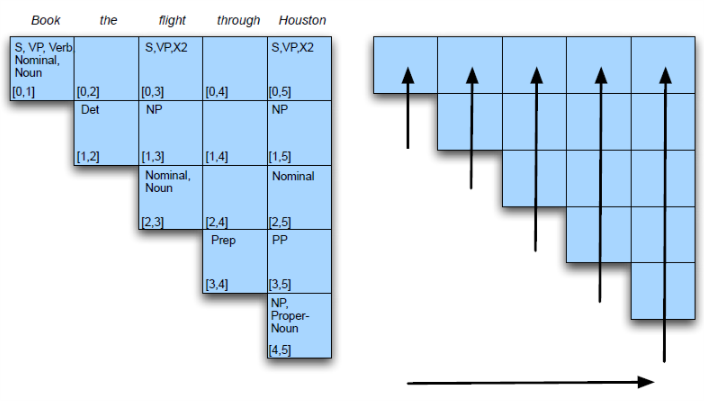
\includegraphics[width=\textwidth]{gfx/cky-beispiel.png} 
\caption{Links: Beispielmatrix für den \textit{CKY}-Algorithmus angewandt auf den Satz \textit{``Book the flight through Houston''}. Rechts: Füllrichtung der Matrix. Beides entnommen aus \cite[S. 473]{nlpGrundlagen}
}	
\label{fig:cky-beispiel}
\end{figure}

\begin{figure} [h]
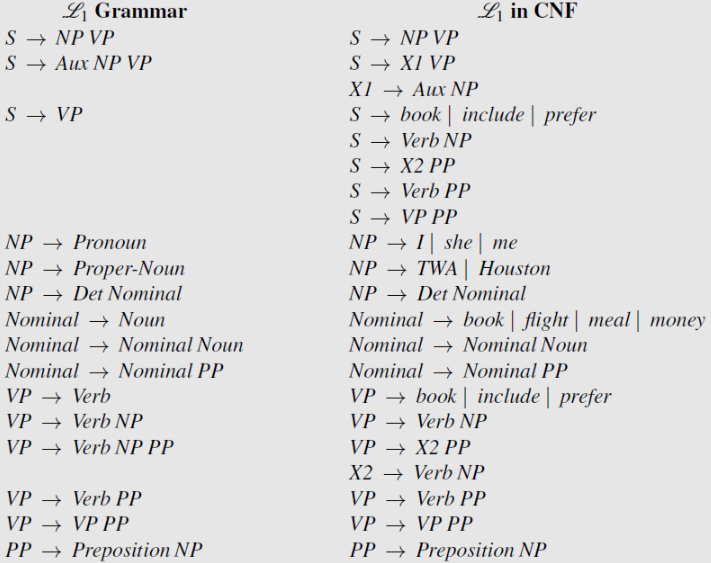
\includegraphics[width=\textwidth]{gfx/grammatik-cky-beispiel.png} 
\caption{Grammatik welche zum Parsen von \textit{``Book the flight through Houston''} verwendet wurde. Links in ursprünglicher Form, rechts in CNF. Entnommen aus \cite[S. 472]{nlpGrundlagen}
}	
\label{fig:cky-beispiel}
\end{figure}

Ohne zusätzliche Informationen gibt die Tabelle nur an, ob ein Satz grammatikalisch korrekt ist. Ein Satz ist korrekt, wenn in Zelle \([0, n]\) das Startsymbol steht. Um die verwendeten Regeln, also den Baum, bzw. die Bäume zur Eingabe zu erhalten, muss der Algorithmus erweitert werden. Die Erweiterung besteht darin, zu jedem Nichtterminal in jeder Zelle zusätzlich zu speichern, aus welchen zwei anderen Nichtterminalen es entstanden ist. Darüber hinaus darf das gleiche Nichtterminal mehrmals in einer Zelle vorkommen, da es aus unterschiedlichen Nichtterminalen entstanden sein kann. Ein Beispiel zur Tabelle in Abbildung \ref{fig:cky-beispiel} ist in Zelle \([0, 5]\) das Symbol \textit{S}. Es gibt drei Möglichkeiten dieses zu erzeugen: 
\begin{align}
& [0, 1]:Verb \; und\; [1, 5]:NP \nonumber \\ & [0, 3]:VP \; und \; [3, 5]:PP \nonumber \\ & [0, 3]:X2 \; und \; [3, 5]:PP \nonumber
\end{align}
Damit ergeben sich für die Eingabe drei verschiedene Syntaxbäume. Diese werden erstellt, indem man die Tabelle, beginnend mit dem jeweiligen Startsymbol, rückwärts durchläuft.

\section{Statistisches Parsen}
\label{sec:nlp:stat-parsen}

In diesem Abschnitt werden Mittel vorgestellt, welche dem Parser helfen sich zwischen mehreren grammatikalisch korrekten Bäumen eines Eingabesatzes zu entscheiden. Hierfür benötigt der Parser für jeden errechneten Baum zusätzlich die Wahrscheinlichkeit, mit welcher dieser semantisch korrekt ist. Das heißt, jede Lösung ist mit einer Wahrscheinlichkeit versehen und es kann diejenige, deren Wert am höchsten ist, als Lösung gewählt werden. 

\subsection{Probabilistische Kontextfreie Grammatiken}
\label{sec:nlp:stat-parsen:pcfg}

Die Anforderung, einem Baum eine Wahrscheinlichkeit zuzuweisen, lässt sich mit dem Konzept der probabilistischen kontextfreien Grammatiken (kurz \textit{PCFG}) umsetzen. Abgesehen von zwei Erweiterungen haben die Produktionen einer \textit{PCFG} die gleiche Form wie die der ursprünglichen kontextfreien Grammatik. Erstens wird jeder Regel eine Wahrscheinlichkeit \textit{p}, mit \( 0 \leq p \leq 1 \), hinzugefügt.
\begin{equation}
A \to \beta  [p]
\end{equation}
Diese gibt an, mit welcher Wahrscheinlichkeit die rechte Seite unter der Vorbedingung der linken Seite auftritt.
\begin{equation}
p := P(A \to \beta | A)
\end{equation}
Es handelt sich um eine bedingte Wahrscheinlichkeit.\\ 
Zweitens muss für jedes Nichtterminal die Summe der Wahrscheinlichkeiten aller seiner Produktionen eins ergeben.
\begin{equation}
\sum_{\beta} P(A \to \beta) = 1
\end{equation}
Die Wahrscheinlichkeit für einen Baum errechnet sich dann durch das Produkt der Wahrscheinlichkeiten aller verwendeten Regeln. Eine Grammatik ist konsistent, wenn die Summe der Wahrscheinlichkeiten aller möglichen Sätze eins ergibt. Inkonsistenz tritt auf, falls es eine Regel der Form \( A \to A \) gibt.\\
Mit dieser neuen Art von Grammatik ergeben sich auch neue Algorithmen zum Berechnen der Bäume. Sowohl der \textit{CKY}- als auch der \textit{Earley}-Algorithmus sind um den Faktor der Wahrscheinlichkeit erweiterbar, wobei der \textit{CKY}-Algorithmus mehr Verwendung findet. \\
Der in Kapitel \ref{sec:nlp:syn-parsen:cky} vorgestellte \textit{CKY}-Algorithmus wird dahingehend erweitert, dass in jeder Zelle für jedes Nichtterminal die zugehörige Wahrscheinlichkeit gespeichert wird. Damit erhält man eine dreidimensionale \( (n+1) \times (n+1) \times V\) Matrix, wobei \textit{V} die Anzahl an Nichtterminalen in der Grammatik, und \textit{n} wie bisher die Anzahl an Wörtern im Satz, ist. \\
Einen Nutzen kann man aus der zugefügten Wahrscheinlichkeit nur dann ziehen, wenn ihr numerischer Wert Sinn ergibt. Um diesen Wert für jede Regel zu berechnen, gibt es zwei Möglichkeiten. Zum einen kann dieser aus einer vollständig annotierten \textit{Treebank} errechnet werden. Hierfür wird jedes Auftreten einer Regel und des entsprechenden Nichtterminals gezählt und dividiert: 
\begin{equation}
P(A \to \beta) = \frac{Anzahl(A \to \beta)}{ \sum_{\gamma} Anzahl(A \to \gamma)} = \frac{Anzahl(A \to \beta)}{Anzahl(A)}
\end{equation}
Die Grammatik wird also anhand der annotierten Sätze der \textit{Treebank} trainiert. Die verwendeten Sätze werden Trainingsdaten genannt. \\
Falls man keine solche \textit{Treebank} zur Verfügung hat, gibt es eine zweite Möglichkeit die Werte der \textit{PCFG} festzulegen. Hierzu arbeitet der Parser einen unannotierter Textkorpus durch und fügt die entsprechenden \textit{Tags} ein. Zu Beginn haben alle Produktionen eines Nichtterminals die selbe Wahrscheinlichkeit. Der Korpus wird iterativ durchlaufen und nach jedem Durchgang werden die Wahrscheinlichkeiten der Regeln angepasst. Dieses Anpassen erfolgt gemäß der ersten vorgestellten Möglichkeit, da zu diesem Zeitpunkt eine annotierte \textit{Treebank} vorhanden ist. Das Verfahren endet, wenn die Wahrscheinlichkeiten konvergieren. \\
Die resultierenden Werte in der Grammatik hängen davon ab, mit welchem Korpus sie berechnet wurden. Hierbei spielen Größe und Textart eine große Rolle. Um beim Parsen eines Textes möglichst gute Ergebnisse zu erhalten, sollte der Parser eine \textit{PCFG} verwenden, welche mit einem Text des selben Genres erstellt wurde. So kann man beispielsweise mit einer \textit{Treebank} aus technischen Handbüchern, unabhängig von ihrer Größe, beim Parsen eines informellen, gesprochenen Dialogs keine guten Ergebnisse erwarten, da sich die Sprache zu sehr unterscheidet.\\ 
Außerdem weist dieses neue Konzept auch zwei Nachteile auf.
Das erste Problem der \textit{PCFG} ergibt sich aus der Kontextfreiheit. Die Wahrscheinlichkeit einer Produktion ist immer gleich, egal an welcher Stelle im Satz sie auftritt. In einer natürlichen Sprache ist das aber im Allgemeinen nicht der Fall. Beispielweise kann die gewählte Produktion einer Nominalphrase abhängig davon sein, ob die Phrase Objekt oder Subjekt des Satzes ist. Da diese Information ohne Weiteres nicht in der Grammatik berücksichtigt werden kann, muss der Mittelwert aus beiden Fällen gebildet werden. Dies führt dazu, dass entweder im Falle des Objekts oder des Subjekts häufig die falsche Regel angewendet wird. \\
Die zweite Schwachstelle ergibt sich daraus, dass die tatsächlichen Wörter nicht einbezogen werden. Als Beispiel hierfür dient die bereits erklärte Anbindungs-Mehrdeutigkeit aus Kapitel \ref{sec:nlp:syn-parsen}. Wiederum wird eine Präpositionalphrase betrachtet, welche entweder an eine Verbal- oder eine Nominalphrase angebunden wird. An welche von beiden hängt allein von der \textit{Treebank} ab. Dort tritt entweder die Produktion \[ VP  \to  \alpha \;\;  NP \;\; PP \] oder die Kombination aus \[ VP  \to  \alpha \;\; NP \] und \[ NP  \to  NP \;\; PP \] häufiger auf. \( \alpha \) steht für eines der hier möglichen Verb-Nichtterminale, welches aber in beide Fällen das selbe ist und deswegen keine Rolle spielt. Wesentlich bessere Resultate sind hier erzielbar, wenn das Verb aus \textit{VP}, das Nomen aus \textit{NP} und die Präposition aus \textit{PP} in die Entscheidungsfindung einbezogen werden. Es kann aus der \textit{Treebank} die Information gewonnen werden, ob die gegebene Präposition sich häufiger auf das Nomen oder das Verb bezieht. Angenommen es gibt eine Präposition, die ausschließlich mit Verben in Verbindung steht. In der \textit{Treebank} sind es nun aber die Nominalphrasen, an welche öfter Präpositionalphrasen gebunden werden. Dann wird die eben angenommene Präposition mit einer \textit{PCFG}, welche mit der \textit{Treebank} errechnet wurde, immer falsch zugeordnet. \\ 
Diese Schwäche der \textit{PCFG} macht sich ebenso bei der Koordinations-Mehrdeutigkeit bemerkbar. Beim Verbinden von Phrasen durch Konjunktionen kann wieder die konkrete Konjunktion und die Beziehung zu den entsprechenden Wörtern der zu verbindenden Phrasen betrachtet werden. Hierzu dient wieder das Beispiel aus Abschnitt \ref{sec:nlp:syn-parsen}: \textit{``old men and women''}. Es könnte eine \textit{Treebank} die Information liefern, dass die Wörter \textit{``men''} und \textit{``women''} per \textit{``and''} öfter direkt miteinander verbunden werden, als dass nur eines von beiden das Adjektiv \textit{``old''} zugeordnet bekommt. \\
Eine mögliche Verbesserung der \textit{PCFG} ergibt sich durch das Erweitern der Nichtterminale um die Information wessen Kind es ist. Es wird ein \textit{NP} als \textit{NP\^{}S} geschrieben, wenn \textit{S} der Elternknoten ist, oder als \textit{NP\^{}VP}, wenn es \textit{VP} ist. Hierdurch ergeben sich zwei neue Regeln in der Grammatik und damit auch zwei neue Wahrscheinlichkeiten. Mit diesem Konzept kann dem Nichtterminal, obwohl die Kontextfreiheit im grammatikalischen Sinne nicht verletzt wird, ein Kontext gegeben werden. Allerdings wird, wenn jedes Nichtterminal für jeden möglichen Elternknoten eine neue Produktion erhält, die Grammatik enorm aufgeblasen. Nebeneffekt dieser neuen Größe ist, dass bei gleich bleibender \textit{Treebank} für jede Regel weniger Trainingsdaten zur Verfügung stehen und damit die erhaltenen Wahrscheinlichkeitswerte ungenauer sind. Für einen gegebenen annotierten Trainings-Korpus muss ein Split-and-Merge Algorithmus ausgeführt werden, der errechnet wie weit eine Aufteilung der Nichtterminale sinnvoll ist.

\subsection{Probabilistische Lexikalisierte Kontextfreie Grammatiken}
\label{sec:nlp:stat-parsen:plcfg}

Ein weiterer Ansatz, um bessere Parserergebnisse zu erhalten, ist das Lexikalisieren der Grammatik. Hierfür muss der Begriff des Kopfes, im Englischen \textit{Head}, eingeführt werden. Die Idee ist, dass jede syntaktische Einheit einen Kopf in Form eines Wortes aus dieser Einheit besitzt. Es wird das Wort genommen, welches ``im Satz am grammatikalisch wichtigsten ist'' \cite[S. 443]{nlpGrundlagen}. 
Für das Finden des richtiges Wortes gibt es verschiedene Schritte. Begonnen wird, indem jedes POS-Nichtterminal sein Kind als \textit{Head} wählt. Dieses Wort wird dann im Baum nach oben weitergegeben. Für jede syntaktische Einheit gibt es Regeln, anhand derer einer der Köpfe der Kinder ausgewählt und als eigener eingesetzt wird. Ein Beispiel ist der lexikalisierte Baum für den Satz \textit{workers dumped sacks into a bin}, dargestellt in Abbildung \ref{fig:lex-tree-dumped-sacks}. 
\\
\begin{figure}
\qtreecentertrue\Tree [.S(dumped) [.NP(workers) [.NNS(workers) workers ] ] [.VP(dumped) [.VDB(dumped) dumped ] [.NP(sacks) [.NNS(sacks) sacks ] ] [.PP(into) [.IN(into) into ] [.NP(bin) [.DT(a) a ] [.NN(bin) bin ] ] ] ] ]
\caption{Lexikalisierter Baum für den Satz \textit{``Workers dumped sacks into a bin''}, entnommen aus \cite[S. 445]{nlpGrundlagen}}
\label{fig:lex-tree-dumped-sacks}
\end{figure}
Zusätzlich zum Kopfwort kann auch noch dessen POS-Tag abgespeichert werden. Somit wird beispielsweise \textit{S(dumped)} zu \textit{S(dumped, VBD)} und \textit{NNS(workers)} zu \textit{NNS(workers, NNS)}. Die Wahrscheinlichkeit der Regel 
\begin{equation}\label{eqn:lexikal-dumped-sacks}
VP(dumped, VBD)  \to  VBD(dumped, VBD) \;\;  NP(sacks, NNS) \;\; PP(into, IN) 
\end{equation}
ergibt sich wieder aus dem Inhalt der \textit{Treebank}, durch die Formel
\begin{equation}
\frac{Anzahl(VP(dumped, VBD)  \to  VBD(dumped, VBD) \;  NP(sacks, NNS) \; PP(into, IN))}{Anzahl(VP(dumped, VBD))} 
\end{equation}
Dieser Wert ist null, wenn der Korpus keinen Satz mit \textit{dumped} \textit{sacks} \textit{into} enthält. Existiert kein Satz in welchem sich \textit{VP(dumped, VBD)} finden lässt, so ist dieser Wert nicht definiert. \\
Aufgrund dieses Problems bedarf es anderer Berechnungsvorschriften, wie zum Beispiel \textit{Collins Model 1}, vorgestellt in \cite{collinsModel}. 
Es wird jede Produktion folgendermaßen betrachtet: \textit{H} ist der Kopf, \( L_i \) sind die Nichtterminale linksseitig und \( R_i \) die rechtsseitig davon. Alle Nichtterminale bleiben weiterhin lexikalisiert. Das Kopfwort wird mit \textit{h} bezeichnet. Damit ergibt sich die Form
\[ A \to L_n...L_1 H R_1...R_m \]
Zusätzlich wird an der Stelle \( L_{n+1} \) und \( R_{m+1} \) das Nichtterminal \textit{STOP} eingefügt, um anzuzeigen, dass hiernach die Regel zu Ende ist. In drei Schritten wird die Wahrscheinlichkeit der Produktion errechnet:
\begin{enumerate}
\item Es wird der Kopf mit der Wahrscheinlichkeit \( P_H(H | A, h) \) generiert.
\item Alle Elemente rechts vom Kopf werden mit \( \displaystyle\prod_{i = 1}^{m+1} P_R(R_i | A, h, H) \), also einschließlich dem \textit{STOP}, generiert.
\item Alle Elemente links von \textit{H} werden mit \( \displaystyle\prod_{i = 1}^{n+1} P_L(L_i | A, h, H) \) generiert.
\end{enumerate}
Für die Regel (\ref{eqn:lexikal-dumped-sacks}) errechnet sich die Wahrscheinlichkeit über
\begin{align}
P & = P_H(VBD|VP, dumped) \nonumber \\ & \times P_R(NP(sacks, NNS)|VP, dumped, VBD) \nonumber \\ & \times P_R(PP(into, IN)|VP, dumped, VBD) \nonumber \\ & \times P_R(STOP|VP, dumped, VBD) \nonumber \\ & \times P_L(STOP|VP, dumped, VBD)
\end{align}
Im Gegensatz zum vorherigen Ansatz muss nicht die Kombination aus \textit{NP(sacks, NNS)}, \textit{PP(into, IN)} und \textit{VBD(dumped, VBD)} vorhanden sein. Es genügt, wenn jedes einzeln, als Kind von \textit{VP(dumped, VBD)}, auf der entsprechenden Seite des \textit{Heads} in der \textit{Treebank} zu finden ist. 
Der Vollständigkeit halber ist außerdem zu erwähnen, dass dieses Modell um die Information der Distanz erweitert wird. Es wird zusätzlich berücksichtigt, wie weit ein Nichtterminal vom Kopf der Regel entfernt ist. 
Außerdem gibt es neben \textit{Model 1} noch zwei weitere Modelle. Diese Modelle bilden die Grundlage für den \textit{Collins Parser}. \cite{collinsModel}